\documentclass{ltjsarticle}
% 数式
\usepackage{amsmath}
% 画像表示
\usepackage{graphicx}
\usepackage{svg}
% 表を使いやすく
\usepackage{tabularx}
% 図の場所を強制
\usepackage{here}
% URL
\usepackage{url}
% ハイパーリンクがつく
\usepackage{hyperref}
% 文章を枠で囲う
\usepackage{ascmac}
% enumerateのラベルを変更可能に
\usepackage{enumitem}
% 外部のファイルからテキストを読み込む
\usepackage{moreverb}
% ソースコードの表示用
\usepackage{listings}
%ソースコードの表示に関する設定
\lstset{
    basicstyle={\ttfamily},
    identifierstyle={\small},
    commentstyle={\smallitshape},
    keywordstyle={\small\bfseries},
    ndkeywordstyle={\small},
    stringstyle={\small\ttfamily},
    frame={tb},
    breaklines=true,
    columns=[l]{fullflexible},
    numbers=left,
    xrightmargin=0\zw,
    xleftmargin=3\zw,
    numberstyle={\scriptsize},
    stepnumber=1,
    numbersep=1\zw,
    lineskip=-0.5ex
}
\renewcommand{\lstlistingname}{リスト}
% 中央揃え(tabularx)
\newcolumntype{C}{>{\centering\arraybackslash}X}
% 左揃え(tabularx)
\newcolumntype{L}{>{\scriptsize\raggedright\arraybackslash}X}
% 右揃え(tabularx)
\newcolumntype{R}{>{\scriptsize\raggedleft\arraybackslash}X}
% 行の中心に配置
\newcommand{\CenterRow}[2]{
    \dimen0=\ht\strutbox%
    \advance\dimen0\dp\strutbox%
    \multiply\dimen0 by#1%
    \divide\dimen0 by2%
    \advance\dimen0 by-.5\normalbaselineskip%
    \raisebox{-\dimen0}[0pt][0pt]{#2}
}


\title{\vspace{-4cm}
制御工学実験Ⅱ テーマ:マイコン基礎応用
}
\author{
    制御情報システム工学科 4年 10番 國安柾希
}

\begin{document}
\maketitle

\subsection*{実施評価}
\begin{tabularx}{\textwidth}{|p{130mm}|C|C|} \hline
    \CenterRow{2}{評価項目} & 自己評価             & 担当評価 \\ \hline
    実験開始までに実験テキストや実験ノートを準備できており,事前課題がある場合は,それに取り組んでいた.
                        & \CenterRow{2}{A} &      \\ \hline
    担当者による指示をよく聞き,不注意による無用な誤りなく安全に実験を行うことができた.
                        & \CenterRow{2}{A} &      \\ \hline
    回路やプログラムを自分で作成し,グループワークの場合は自らの役割を全うするなど,課題に対して積極的に取り組むことができた.
                        & \CenterRow{2}{A} &      \\ \hline
    与えられた課題を時間内に達成し,結果を正確に記録または出力できた. \par
                        & \CenterRow{2}{B} &      \\ \hline
    使用器具の後片付けや実験場所の清掃をきちんと行った. \par
                        & \CenterRow{2}{A} &      \\ \hline
\end{tabularx}

\subsection*{レポート評価}
\begin{tabularx}{\textwidth}{|p{130mm}|C|C|} \hline
    \CenterRow{2}{評価項目} & 自己評価             & 担当評価 \\ \hline
    章立ては適切であり,それぞれの章における記載内容は自作のものである.引用がある場合は,その旨を明記している.
                        & \CenterRow{2}{A} &      \\ \hline
    図・表の書き方は裏面の要領に準じており,自作のものである.(担当者が許可しない限り,指導書の図すら引用してはいけない)
                        & \CenterRow{2}{A} &      \\ \hline
    使用器具や実験環境について,実験結果を再現するのに十分な情報を記載している. \par
                        & \CenterRow{2}{A} &      \\ \hline
    課題に関する計測結果や出力結果を整理して記載し,結果に対する独自の考察を述べている.
                        & \CenterRow{2}{A} &      \\ \hline
    研究課題に取り組み,適切な参考文献を基に答えを導き出している. \par
                        & \CenterRow{2}{C} &      \\ \hline
\end{tabularx}

\begin{center}
    \begin{tabularx}{100mm}{|C|C|C|} \hline
        実施点\par(50)  & レポート点\par(50) & 合計点\par(100) \\ \hline
        \ \par\ \par &               &              \\ \hline
    \end{tabularx}
\end{center}

\newpage
\section{実験目的}

今までの実験では,PCで作成したプログラムをArduinoに書き込んで実行してきた.しかし,Arduinoへの書き込みのみでは,要求する動作が複数ある場合,選択することが困難になる場合がある.
それを解決するために,今回の実験では,Arduinoのプログラムを書き込んだ後にArduinoとPC間でシリアル通信を行って,PCからコマンドを送信してハードウエアの制御を行う.
また,Webサイトから必要な情報を収集し実際に実装することで,具体的な知識やスキルを身に着け,そのシステム構築を通して,PCとArduinoの連携を利用した,より複雑なシステムの構築方法を身に着ける.

% タイトルは自分で考える
% 「実験目的」で出したキーワードについて,数式やフローチャート,図や表を利用して詳細な仕組みを説明する.

\section{構築した組み込みシステム}
\subsection{実験課題}
以下の条件を満たすシステムを構築する
% 半固定抵抗のつまみの角度(位置)に対応してサーボモータの
% 角度を変える(自動車のパワーステアリングのイメージ)
\begin{itemize}
    \item 入力:シリアル通信(Rx),半固定抵抗(10kΩ)
    \item 出力:シリアル通信(Tx),赤黄LEDを各1個,サーボモータ
    \item 動作:\begin{enumerate}
              \item PCからコマンド操作(シリアルモニタから文字列を送信して操作)

                    “r,ooo”: 赤色LEDをoooの明るさにする(oooは0-255の整数)

                    “y,ooo”: 黄色LEDをoooの明るさにする

                    “w,ooo,OOO”: 赤色LEDをooo,黄色LEDをOOOの明るさにする

                    “s”: 赤色LEDと黄色LEDの現在の明るさをPCに送る
              \item 半固定抵抗のつまみの角度(位置)に対応してサーボモータの角度を変える(自動車のパワーステアリングのイメージ)
          \end{enumerate}
\end{itemize}

\subsection{実験結果}
作成したシステムの実際の回路,回路図を図\ref{fig:task1-1},\ref{fig:task1-2},プログラムをリスト\ref{lst:task1prog}に示す.\\\\
\begin{figure}[h]
    \centering
    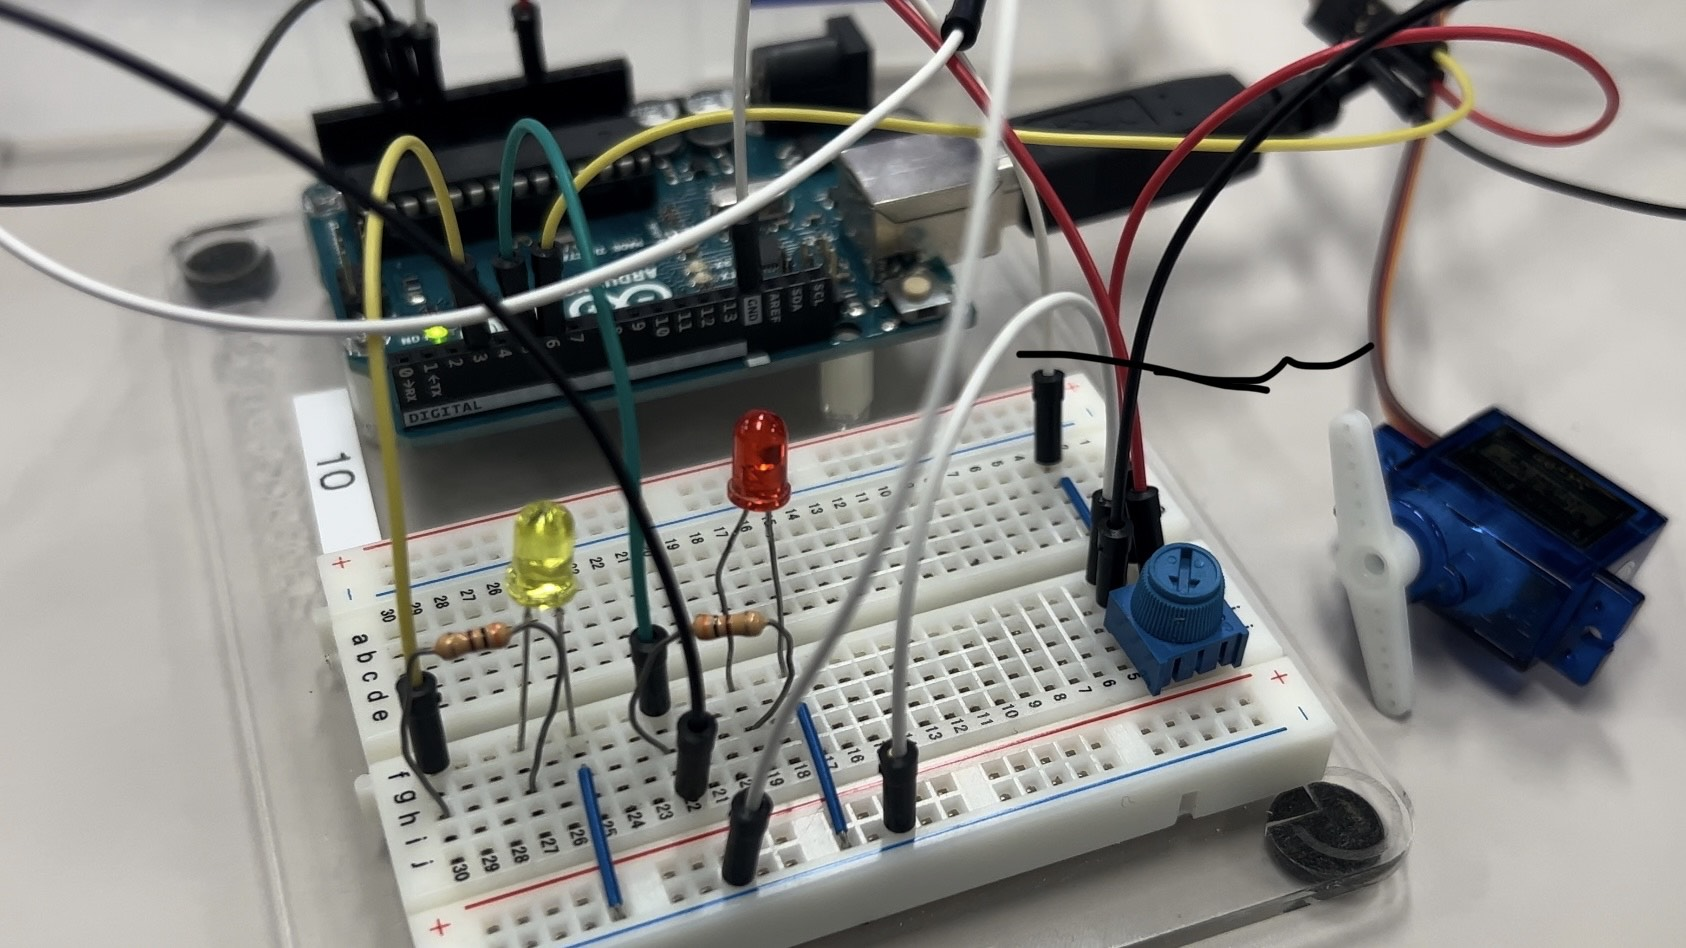
\includegraphics[width=\linewidth]{figures/task1.jpg}
    \caption{実際の回路}
    \label{fig:task1-1}
\end{figure}

\begin{figure}[h]
    \centering
    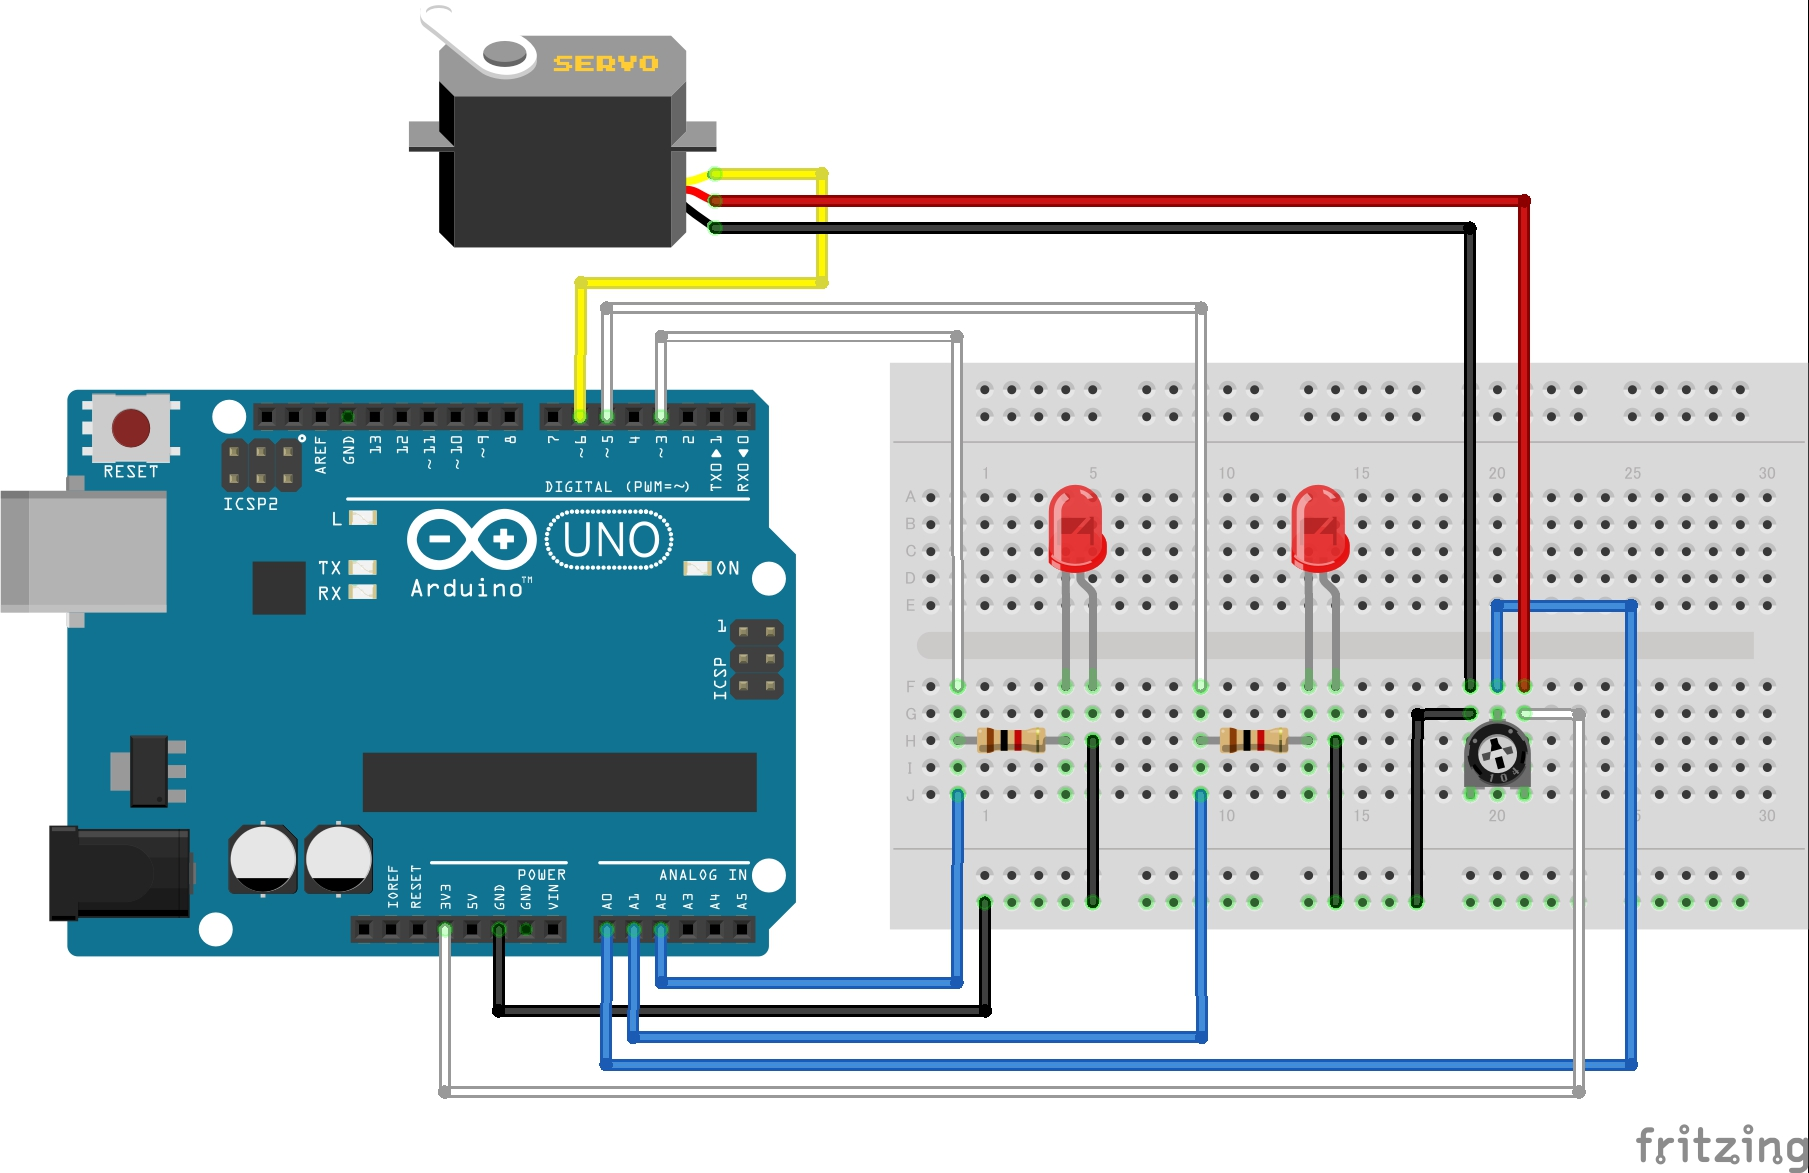
\includegraphics[width=\linewidth]{figures/0628fig.jpg}
    \caption{作成した回路の回路図}
    \label{fig:task1-2}
\end{figure}
\clearpage

\lstinputlisting[caption=課題のプログラム,label=lst:task1prog]{src/task0607.ino}

\subsubsection*{ハードウエアについて}
今回の課題では図\ref{fig:task1-1},\ref{fig:task1-2}のような回路を作成した.
図\ref{fig:task1-2}より,Arduinoのデジタルピン6番にサーボモータを接続し,デジタルピン5番に赤色LED,デジタルピン3番に黄色LEDを接続した.
また,状態を読み取るために,A2ピンに赤色LED,A2ピンに黄色LED,A0ピンにサーボモーターを接続した.

\subsubsection*{ソフトウェアについて}
今回の課題では,リスト\ref{lst:task1prog}のようなプログラムを作成した.
まず,1~7行目で使用するモジュールのインポート,記号定数の定義を行った.
11~22行目のsetup関数では,Serial.begin()関数によりシリアル通信の初期化を行い,サーボモータの動作に使用するピン,LEDの点灯に使用するピンを,pinMode(),servo.attach()関数を用いて設定した.
また,serbo.attach()関数では,第一引数にサーボモータのピン番号,第二,三引数にパルス幅を指定することが出来る.
次に,24~63行目までのloop関数では,25~28行目まででサーボモータの処理,30~62行目まででLEDの処理を行った.


サーボモータについては,26行目でA0ピンからの入力を読み取り,27行目で読み取った値をmap()関数を用いて,500~2400までの整数値に変換し,serbo.writeMicroseconds()関数を用いてサーボモータが接続されているD6端子に出力している.
また,LEDについては,32,33行目でSerial.readString()関数を用いてシリアル通信からの入力を読み取り,35~61行目で入力されたコマンドを判定し,コマンドに応じた動作を行っている.
45~52行目のコマンドwについては,コンマの添え字を求め,substring(),toInt()関数を用いて,コンマの前後の値を取り出し,それぞれの値をanalogWrite()関数を用いて,5・3ピンへ出力している.
53~60行目のコマンドsについては,analogRead()関数を用いて,A1,A2ピンからの入力を読み取りmap()関数を用いて値を変換し,Serial.print()関数を用いて,読み取った値をシリアル通信でPCに送信し表示している.


\section{考察}

\subsection*{PWM制御について}
%PWM(PulseWidthModulation)制御についてレポート調で説明する.
PWM(PulseWidthModulation)制御とは,パルス波形を出力し,デジタル信号を用いてアナログ信号を表現する制御方法である.
PWM制御では,デジタル信号のON時間とOFF時間の割合を変化させることで,アナログ信号を表現する.
ON時間とOFF時間の割合をデューティ比と呼び,デューティ比が大きいほど,アナログ信号の値が大きくなる.\\
また,PWM制御では,デジタル信号の周波数も重要である.
デジタル信号の周波数が高いほど,アナログ信号の値が滑らかになるが,デジタル信号の周波数が高いほど,処理にかかる時間が長くなるため,デジタル信号の周波数は,アナログ信号の値の滑らかさと処理時間のバランスを考慮して設定する必要がある.

\subsection*{Aruduinoの端子について}
%LEDの点灯システムの実装時にPWM制御に対応していないピンを使用してしまい,255と入力した際にしか点灯しないというミスを犯してしまってLEDの点灯がうまくいかなかった旨を記述し,端子の種類や可能な処理について説明する.
Arduinoの端子について考察する.
Arduinoの端子には,デジタルピンとアナログピンが存在し,デジタルピンは,HIGH(5V)とLOW(0V)の2つの状態を表現することができる.また,PWM制御に対応しているピンと非対応のピンが存在する.
アナログピンは,0V~5Vの範囲の電圧を表現することができ,Arduino UNOなどのマイコンはHighかLowしか認識ができないが,A/D変換機能を使うことでアナログ電圧をデジタル信号に変換して認識することがである.\cite{key}
今回の課題では,LEDの点灯にデジタル5・3ピンを使用したが,最初は9・8ピンを使用していた.
しかし,8ピンはPWM制御に対応していないため,255と入力した際にしか点灯しなかった.ピン番号の先頭についている” ~ ”はPWM制御に対応していることを表しているため,LEDの明るさの調整をする場合はPWM制御に対応しているピンに接続しないと明るさを調整することが出来ないことに注意が必要である.

\subsection*{割り込みについて}
%マイコン基礎応用.pdfを参照し,割り込み処理について記述する.
今回の実験では研究課題に取り組む時間を確保できなかったため,実際に実装することは出来なかったが,割り込み処理について調査した.
割り込み処理とは,マイコンが処理を行っている最中に,外部からの信号を受け取り,その信号に応じた処理を行うことである.
割り込み処理を行うと,現在実行してい処理を中断し,ほかのプログラムを実行する.そして,割り込んだ処理が終了すると,中断していた処理を再開する.
Arduinoでは主に2種類の割り込み処理が存在する.

\begin{itemize}
    \item タイマ割り込み

          一定時間ごとに割り込み処理を行う.
    \item 外部割り込み

          Arduinoに接続されているスイッチやセンサなどに変化があった場合に処理を行う.
\end{itemize}

また,Arduinoで割り込み処理を行うためには,割り込み処理を行うピンを設定し,そのピンに信号が入力された際に,割り込み処理を行う関数を呼び出すように設定する必要がある.
割り込み処理を行う関数は,void setup()関数内でattachInterrupt()関数を用いて設定する.
attachInterrupt()関数は,引数に割り込み処理を行うピン番号,割り込み処理を行う関数,割り込み処理を行うタイミングを指定する.



\section{感想}

ピンを間違えているためLEDの点灯がうまくいっていないことに気づくまでに時間がかかってしまったため,しっかりと取り扱う機材のピンの種類などの下調べをしなければいけないなと痛感した.
また,今まではArduinoにコードの書き込みを行った後にPC側からの操作というのはあまりしてこなかったが,今回の実験ではPC→Arduino→ハードウエアという操作を実装できたため,一気に世界が広がったような気がした.
現在リベラルアーツ実践の授業において,Arduinoなどのマイコンを利用したシステムの構築を行っているのでそこでも今回の経験が生かせると思う.

\begin{thebibliography}{9}
    \bibitem{key} ArduinoUNOのピン配置と役割, なかしー, \url{https://miraiworks.org/?p=5655}, (参照日 2023/6/25)
    \bibitem{key} Arduinoの割り込み機能とは?, なかしー, \url{https://miraiworks.org/?p=5765}, (参照日 2023/6/25)
\end{thebibliography}
\end{document}
